% !TeX root = demo.tex

\chapter{Theoretical of foundations of classical statistical mechanics}

\section{Overview}

It's statistical mechanics' job to communicate between macroscopic thermodynamics and microscopic laws of motion. Thermodynamics is a phenomenological theory which makes no reference to the microscopic constituents of matter; however, we can rationalize thermodynamics based on microscopic mechanical laws illustrated in chapter 1. But problems emerge:
\begin{itemize}
	\item macroscopic systems possess an enormous number of degree of freedom, or number of particles;
	\item in real-world systems, the interactions between particles are highly nontrivial;
	\item \textit{Loschmidt's paradox}: microscopic mechanical laws are "inherently reversible", while the second law of thermodynamics prescribes a direction of time.
\end{itemize}
People then realized that macroscopic properties of a system do not depend strongly on the motion of every particle, but rather on gross averages that "wash out" microscopic details. 

The principal conceptual breakthrough is that of an \textit{ensemble}, which refers to a collection of systems that share common macroscopic properties. This chapter is mainly about this genius idea.

\section{The laws of thermodynamics}

Here are some concepts.
\begin{itemize}
	\item The thermodynamic system is a macroscopic system. The rest of the universe is called its surroundings.
	\item \textit{Isolated system}: no heat or material is exchange between a system and its surroundings.
	\item A thermodynamic \textit{state} is specified by all thermodynamic parameters (like $p, V, T$) provided experimentally.
	\item The \textit{equation of state} of a system is 
	\item \textit{Thermodynamic transformation}: 
	\item \textit{Thermodynamic equilibrium}: thermodynamic state doesn't change in time.
	\item \textit{State function}:
	\item \textit{Work}: 
		\begin{equation}
			\md W_{rev}=-p\md V+\mu\md n
		\end{equation}
		$\mu$ is called \textit{chemical potential}.
	\item \textit{Heat}:
		\begin{equation}
			\md Q_{rev}=C\md T
		\end{equation}
\end{itemize}

\subsection{The first law of thermodynamics}


\begin{equation}
	\Delta E=\Delta Q+\Delta W
\end{equation}

$W_{irrev}>W_{rev}$

$\Delta E_{uni}=\Delta E_{sys}+\Delta E_{sur}$

\subsection{The second law of thermodynamics}

\subsubsection{The Carnot cycle}
\begin{figure}[!h]
	\centering
	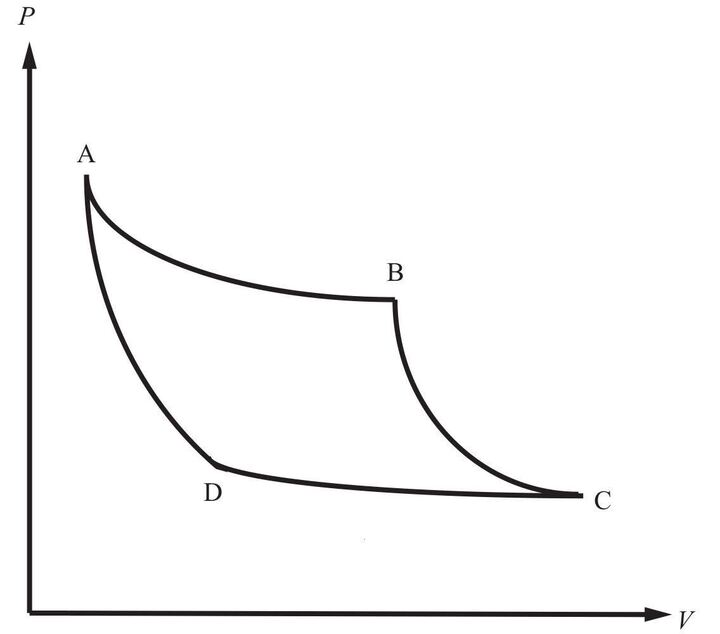
\includegraphics[width=0.6\linewidth]{figure/2.3-carnot}
	\caption{The Carnot cycle}
	\label{fig:2}
\end{figure}


\subsubsection{The second law}


\subsection{The third law of thermodynamics}

Alternative statement: $T=0$ can never be physically reached.


\section{The ensemble concept}





\section{Overview}
\section{Overview}
\section{Overview}
\section{Overview}
\section{Overview}

\section*{Summary of chapter}

\begin{itemize}
	\item 
	\item 
\end{itemize}